% Background

% Main chapter title
%\chapter[toc version]{doc version}
\chapter{Background}

% Short version of the title for the header
%\chaptermark{version for header}

% Chapter Label
% For referencing this chapter elsewhere, use \ref{ChapterTemplate}
\label{Background}

This chapter will cover the concepts needed to contextualize and understand the \ac{ucttp} and the algorithms used to obtain the final result, namely the \ac{mcts} and \ac{hc} algorithms.

%\section Terminology

\section{Combinatorial Optimization Problems}

Finding a solution for maximizing or minimizing a value is common in several real world problems. These problems often require searching for the optimal solution from a finite set of possibilities. They are characterized by their discrete nature and the challenge of finding optimal solutions in large search spaces.

\acp{cop} arise in various fields, such as artificial intelligence, machine learning, auction theory, applied mathematics, and so on. Some well-known \acp{cop} include Knapsack Problem, Traveling Salesman Problem, and Graph Coloring. 

To solve these problems, various algorithmic techniques are used, including:
\begin{itemize}
\item \textbf{Exact algorithms:} Guarantee optimal solutions by exhaustively exploring the solution space. However, they can be computationally expensive, especially for large and complex problems, because their complexity often grows exponentially.
\item \textbf{Approximation algorithms:} Produce provably near-optimal solutions, providing a quantifiable measure of how far the solution might diverge from the best possible one, making them valuable for problems where exact solutions are infeasible.
\item \textbf{Heuristic algorithms:} Focus on practicality and efficiency by finding good solutions within a reasonable time frame. While they do not ensure optimality, they are often effective for solving large-scale problems. This type of algorithms will be the primary focus of this dissertation.
\end{itemize}

\section{University Course Timetabling Problem}
%\subsection{Educational Timetabling}
\ac{ucttp} is a NP-hard \ac{cop} that involves allocating events, rooms, lecturers, and students to weekly schedules while meeting certain predefined constraints. It falls under the broader category of educational timetabling, which also includes other challenging problems such as examination timetabling. 

Due to the size and complexity of the problem, obtaining an optimal solution in usable time is typically infeasible. Therefore, it is necessary to employ robust optimization techniques.

\subsection{Curriculum-Based and Post-Enrollment Course Timetabling}

\ac{ucttp} can be categorized into two main types:

\begin{itemize}
\item \textbf{Curriculum-Based Course Timetabling (CB-CTT):} Courses are grouped into predefined curricula, ensuring that no student or lecturer is allocated to overlapping courses within their curriculum. \ac{fcup}'s timetables generation fit into this approach.

\item \textbf{\ac{pe-ctt}:} Events are scheduled after students enroll in their courses, taking into account their preferred event combinations while minimizing conflicts.
\end{itemize}

These two approaches differ significantly in terms of timing, flexibility, and constraints. \ac{pe-ctt} is performed after the student has enrolled in their courses, while \ac{cb-ctt} is performed first. \ac{pe-ctt} adjusts to the student choices, providing greater flexibility, while \ac{cb-ctt} follows a more rigid and predefined structure. Furthermore, \ac{pe-ctt} often involves more complex constraints due to diverse student preferences, while \ac{cb-ctt} deals with more predictable patterns. As a result, \ac{pe-ctt} is appropriate for institutions with a flexible course enrollment, while \ac{cb-ctt} is ideal for institutions with fixed curricula.

\subsection{Constraints}
%How can a university/school schedule its classes to make the best use of teachers and classrooms without conflicts?
In the context of \ac{ucttp}, constraints are often divided into two different types:
\begin{itemize}
\item \textbf{Hard constraints:} Ensure the feasibility of the timetable and must be strictly satisfied. Typically, a hard constraint includes avoiding overlapping events for the same student or a lecturer. 
\item \textbf{Soft constraints:} Represent preferences to improve the quality of the solution without being mandatory. An example of a soft constraint is minimizing gaps in students' timetables to ensure a more compact timetable.
\end{itemize}

\section{International Timetabling Competition (ITC)}

Since 2002, the \ac{patat}\footnote{https://patatconference.org/communityService.html} has supported timetabling competitions to encourage research in this field. There have already been five \ac{itc}, but only three of them have focused on university timetables.

\subsection{Benchmark datasets}

\ac{itc} provides benchmark datasets that serve to evaluate timetable algorithms. %The most relevant dataset for the \ac{ucttp} is the \ac{itc-2007} dataset, which %presents real-world constraints and objectives commonly found in academic scheduling. These datasets help researchers compare the performance of different algorithms on the same problem instances, ensuring fair and reproducible results.

\section{Monte Carlo Tree Search}

\ac{mcts} is a decision-making algorithm that has been successfully applied in a variety of optimization problems with a huge search space. The algorithm has proven to be particularly effective in games such as Go and Chess, where the algorithm can even outperform the best human players.

\subsection{Phases}
%TODO \cite{browne_survey_2012}

\begin{figure}
      \centering
      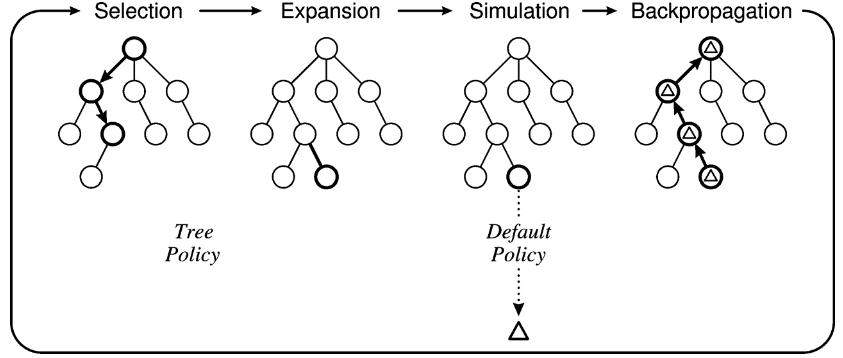
\includegraphics[width=0.7\columnwidth]{Background/MCTS_approach.png}
      \caption[MCTS approach]
      {One MCTS iteration \cite{browne_survey_2012}}
      \label{fig:mcts_approach}
\end{figure}

The algorithm consists of four phases, as illustrated in Figure \ref{fig:mcts_approach}  \cite{browne_survey_2012}. These phases are repeated for a predefined number of iterations or until a computational budget (such as time or memory) is reached. The phases are as follows:

\begin{enumerate}
	\item \textbf{Selection:} The tree is traversed from the root node until it finds a node that is not completely expanded, i.e., a non-terminal node with unvisited children. The selection is guided by a policy that balances exploration and exploitation. Typically, the policy used is \ac{uct}, which selects nodes that maximize formula \ref{uct_formula}.
	 
	\begin{equation}
	UCT = \overline{X_i} + 2C\sqrt{\frac{2\ln{n}}{n_i}},\label{uct_formula}
	\end{equation} where \(\overline{X_i}\) is the total reward of all playouts through this state by the number of visits, \(C\) is a constant greater than zero (typically \sqrt{2}), \(n_i\) is the number of visits of child node \(i\), and \(n\) is the number of visits of the parent node.
    \item \textbf{Expansion:} One or more child nodes are added to the node previously reached in the selection phase.
    \item \textbf{Simulation:} From the newly added node(s), a simulation is performed according to a default policy, which may include random moves until a terminal node is reached.
    \item \textbf{Backpropagation:} The simulation result is then propagated back through the traversed nodes, where the number of visits and the average reward for each node are updated until it reaches the root.
\end{enumerate}

\section{Local Search}

\subsection{Hill Climbing}

%\subsection{Reactive Programming}

%\subsubsection{Elm}

\section{Previous Work}


